\section*{Question 2}

\begin{custombox}[label={box:Q2}]{Question 2}
	Using the $E1$ dataset, fit a Regression line and generate detailed regression output \textbf{using the built-in Regression functionality of the spreadsheet.} Show the Regression output in your report. It should include the regression coefficients, their associated standard errors, $p$-values, confidence intervals, the $F$-statistic, and $R^2$ values. (All spreadsheets create detailed Regression output – some provide a dialog based UI to do it, while in some others appropriate function(s) have to be used.)
\end{custombox}

I fitted a regression line to the dataset $(y, x)$ using the built-in Regression functionality of the spreadsheet. The regression output is shown in the following figure.

\begin{figure}[H]
	\centering
	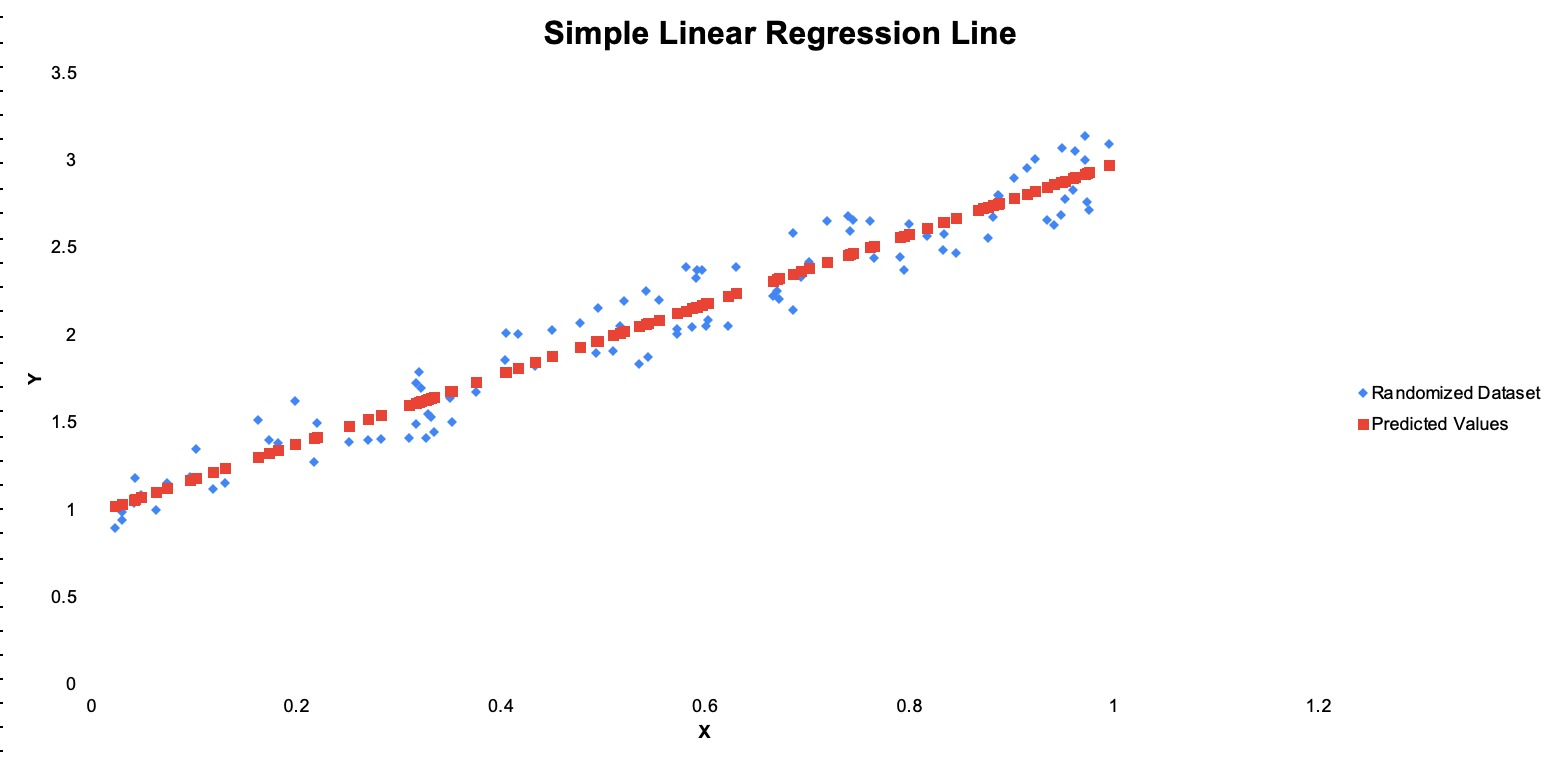
\includegraphics[width=0.8\textwidth]{Images/Q1_2.jpeg}
	\caption{Regression output}
	\label{fig:Q2}
\end{figure}

This is the regression output of the dataset $(y, x)$:

\begin{figure}[H]
	\centering
	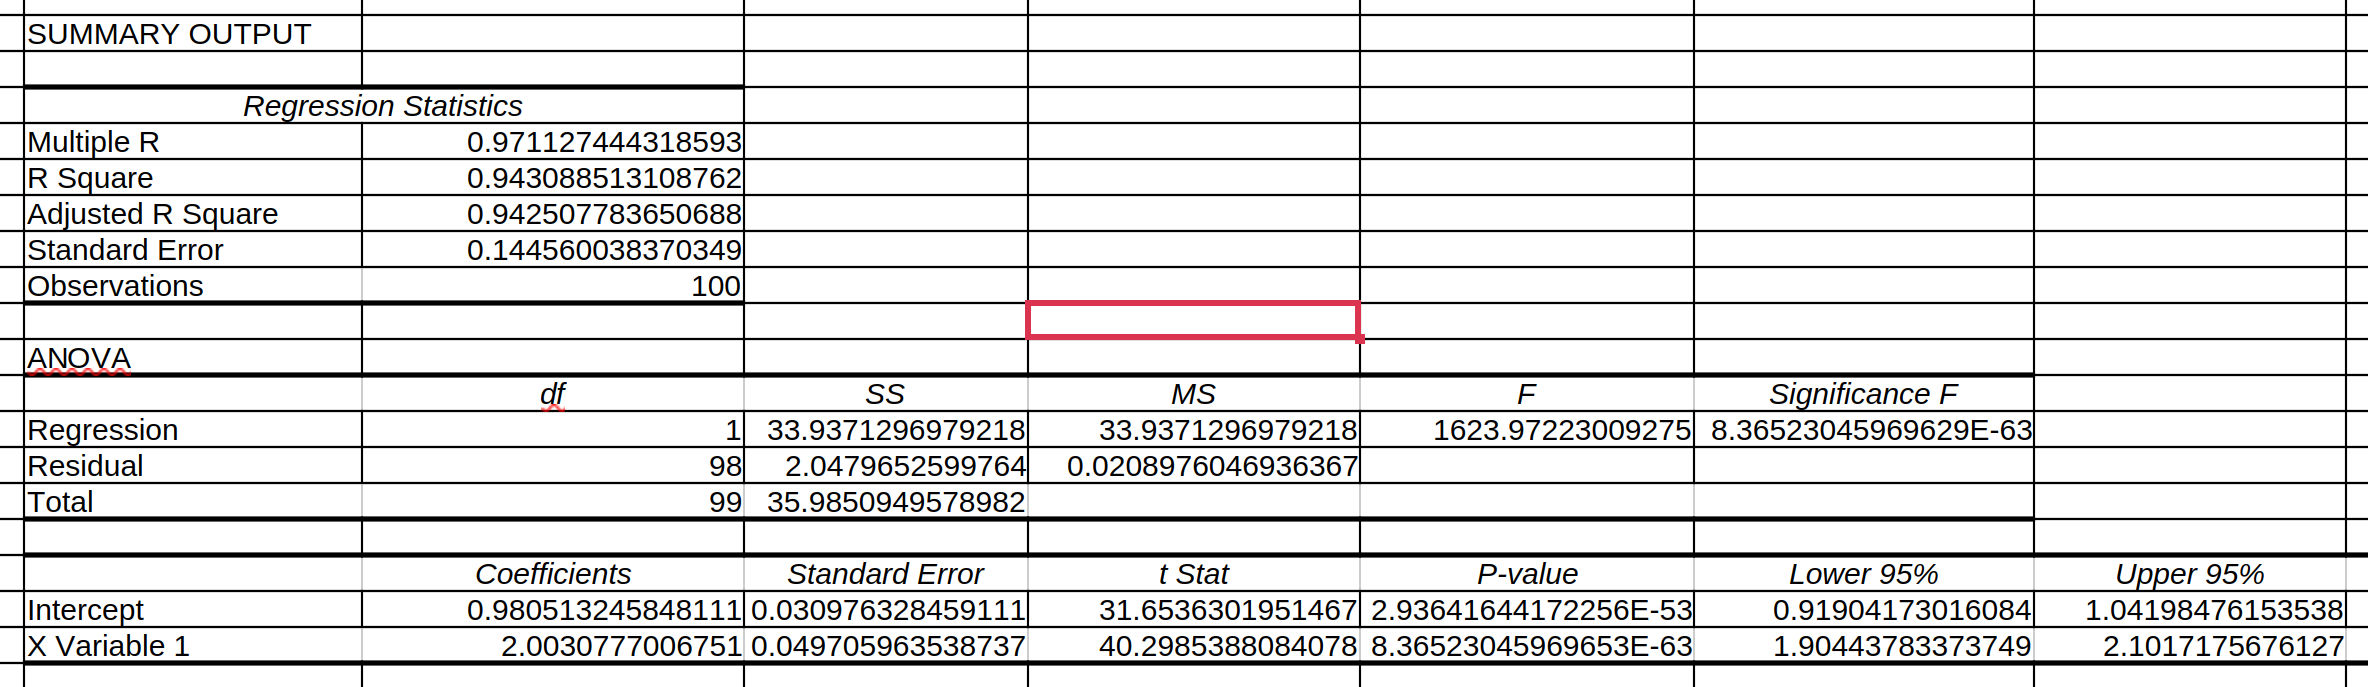
\includegraphics[width=\textwidth]{Images/Q2_1.png}
	\caption{Statistics Related to the Regression}
	\label{fig:Q2_1}
\end{figure}

\clearpage

These are the predicted values of $y$ based on the regression line, also known as $\widehat{y_i}$:

\begin{figure}[H]
	\centering
	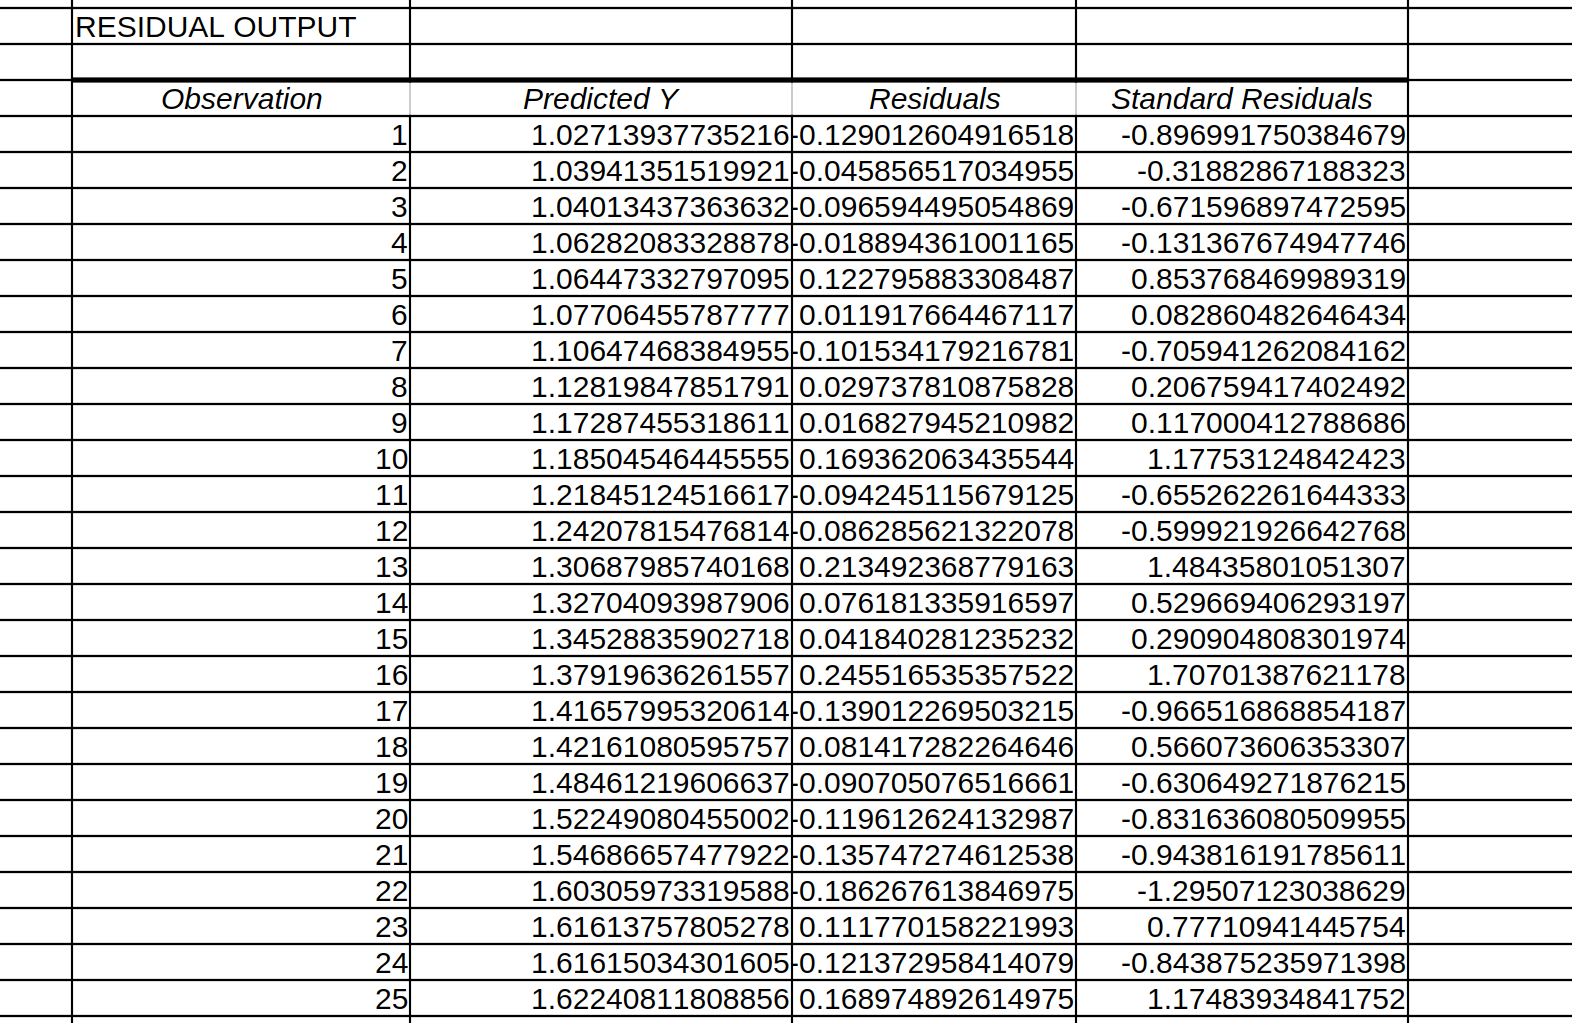
\includegraphics[width=0.8\textwidth]{Images/Q2_2.png}
	\caption{Predicted values of $y$, $\widehat{y_i}$, only 25 shown here}
	\label{fig:Q2_2}
\end{figure}

These are the standard errors obtained from the regression output:

\begin{figure}[H]
	\centering
	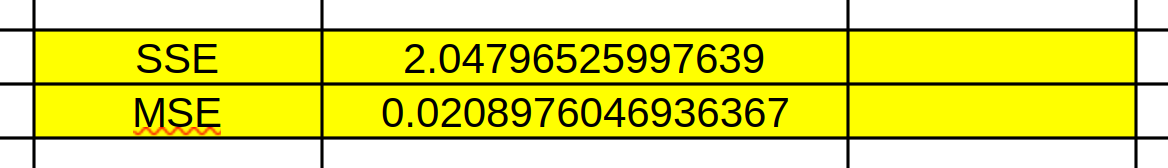
\includegraphics[width=0.8\textwidth]{Images/Q2_3.png}
	\caption{Standard Errors (SSE \& MSE) of the regression}
	\label{fig:Q2_3}
\end{figure}

\clearpage


